\begin{figure}
    \centering
    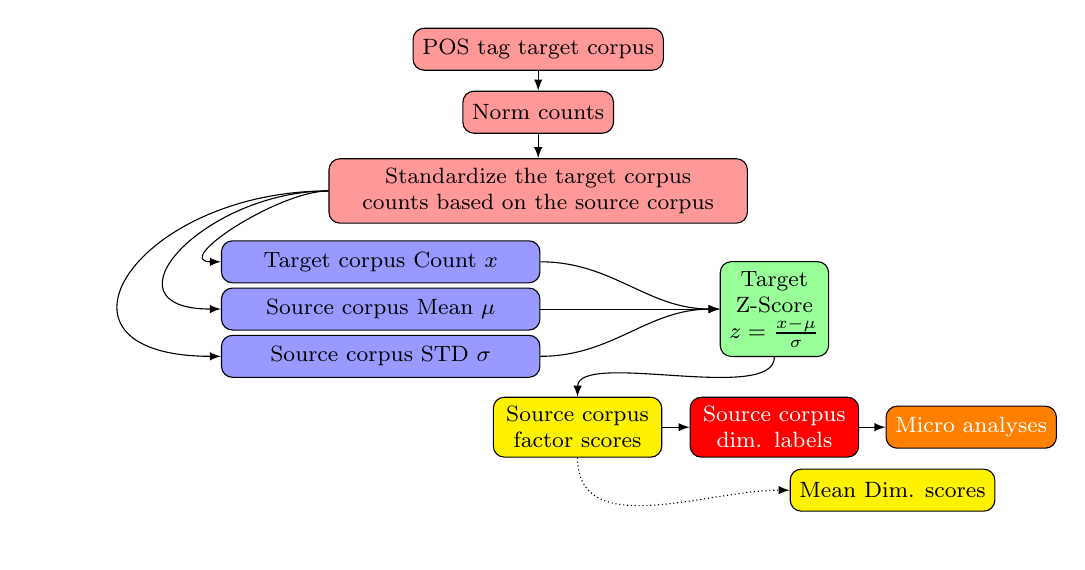
\begin{tikzpicture}
        %\tikzstyle{block} = [rectangle, rounded corners, text=black, text centered, draw=black, minimum height=.3in]
        \tikzstyle{block} = [rectangle, rounded corners, text=black, text centered, draw=black,font=\footnotesize, minimum height=.21in]
        \tikzstyle{line} = [-latex,draw=black,line width=.4]
        \node[block,fill=red!40,text=black] (tag) at (5,3) {POS tag target corpus};
        \node[block,fill=red!40,text=black] (norm) at (5,2.2) {Norm counts};
        \node[block,fill=red!40,text=black, text width=2in] (score1) at (5,1.2) {Standardize the target corpus counts based on the source corpus};
        \node[block,fill=blue!40,text=black, text width=1.5in] (count) at (3,.3) {Target corpus Count $x$};
        \node[block,fill=blue!40,text=black, text width=1.5in] (mean) at (3,-.3) {Source corpus Mean $\mu$};
        \node[block,fill=blue!40,text=black, text width=1.5in] (std) at (3,-.9) {Source corpus STD $\sigma$};
        %\node[block,fill=blue!40,text=black] (comm) at (1,-.2) {Commun.};
        \node[block,fill=green!40,text=black,align=center] (zscore) at (8,-.3) {Target \\ Z-Score \\ \( z = \frac{{x - \mu}}{{\sigma}} \)};
        %\node[block,fill=green!40,text=black] (load) at (7,-.2) {Drop weak loadings};
        %\node[block,fill=green!40,text=black] (standard) at (7,-1) {Standardize counts};
        \node[block,fill=yellow,text=black, text width=.75in] (scores) at (5.5,-1.8) {Source corpus factor scores};
        \node[block,fill=red,text=white, text width=.75in] (labels) at (8,-1.8) {Source corpus dim. labels};
        \node[block,fill=orange,text=white] (analyze) at (10.5,-1.8) {Micro analyses};
        \node[block,fill=yellow,text=black] (dimscores) at (9.5,-2.6) {Mean Dim. scores};
        \draw[line] (tag) to (norm);
        \draw[line] (norm) to (score1);
        \draw[line, densely dotted] (scores) to[in=180,out=270] (dimscores);
        %\draw[line,densely dashed] (standard) to (labels);
        %\draw[line,loosely dashed] (standard) to (labels);
        \draw[line] (score1) to[in=180,out=180,looseness=1] (count);
        \draw[line] (score1) to[in=180,out=180,looseness=2] (mean);
        \draw[line] (score1) to[in=180,out=180,looseness=2.5] (std);
        \draw[line] (count) to[in=180,out=0] (zscore);
        \draw[line] (mean) to[in=180,out=0] (zscore);
        \draw[line] (std) to[in=180,out=0] (zscore);
        \draw[line] (zscore) to[in=90,out=270,looseness=.6] (scores);
        \draw[line] (scores) to[in=180,out=0] (labels);
        \draw[line] (labels) to (analyze);
        %\draw[line] (zscore) to[out=180,in=90] (0,-1.5) to[out=270,in=180] (scores);
    \end{tikzpicture}
    \caption{Análise Multidimensional Aditiva \citep[Original em língua inglesa]{biberVariationEnglishMultiDimensional2001, berbersardinhaAddingRegistersPrevious2019}}
    \label{fig:additive_md_analysis_ptbr}
\end{figure}
